
%% bare_conf.tex
%% V1.4b
%% 2015/08/26
%% by Michael Shell
%% See:
%% http://www.michaelshell.org/
%% for current contact information.
%%
%% This is a skeleton file demonstrating the use of IEEEtran.cls
%% (requires IEEEtran.cls version 1.8b or later) with an IEEE
%% conference paper.
%%
%% Support sites:
%% http://www.michaelshell.org/tex/ieeetran/
%% http://www.ctan.org/pkg/ieeetran
%% and
%% http://www.ieee.org/

%%*************************************************************************
%% Legal Notice:
%% This code is offered as-is without any warranty either expressed or
%% implied; without even the implied warranty of MERCHANTABILITY or
%% FITNESS FOR A PARTICULAR PURPOSE! 
%% User assumes all risk.
%% In no event shall the IEEE or any contributor to this code be liable for
%% any damages or losses, including, but not limited to, incidental,
%% consequential, or any other damages, resulting from the use or misuse
%% of any information contained here.
%%
%% All comments are the opinions of their respective authors and are not
%% necessarily endorsed by the IEEE.
%%
%% This work is distributed under the LaTeX Project Public License (LPPL)
%% ( http://www.latex-project.org/ ) version 1.3, and may be freely used,
%% distributed and modified. A copy of the LPPL, version 1.3, is included
%% in the base LaTeX documentation of all distributions of LaTeX released
%% 2003/12/01 or later.
%% Retain all contribution notices and credits.
%% ** Modified files should be clearly indicated as such, including  **
%% ** renaming them and changing author support contact information. **
%%*************************************************************************


% *** Authors should verify (and, if needed, correct) their LaTeX system  ***
% *** with the testflow diagnostic prior to trusting their LaTeX platform ***
% *** with production work. The IEEE's font choices and paper sizes can   ***
% *** trigger bugs that do not appear when using other class files.       ***                          ***
% The testflow support page is at:
% http://www.michaelshell.org/tex/testflow/



\documentclass[conference]{IEEEtran}
% Some Computer Society conferences also require the compsoc mode option,
% but others use the standard conference format.
%
% If IEEEtran.cls has not been installed into the LaTeX system files,
% manually specify the path to it like:
% \documentclass[conference]{../sty/IEEEtran}





% Some very useful LaTeX packages include:
% (uncomment the ones you want to load)


% *** MISC UTILITY PACKAGES ***
%
%\usepackage{ifpdf}
% Heiko Oberdiek's ifpdf.sty is very useful if you need conditional
% compilation based on whether the output is pdf or dvi.
% usage:
% \ifpdf
%   % pdf code
% \else
%   % dvi code
% \fi
% The latest version of ifpdf.sty can be obtained from:
% http://www.ctan.org/pkg/ifpdf
% Also, note that IEEEtran.cls V1.7 and later provides a builtin
% \ifCLASSINFOpdf conditional that works the same way.
% When switching from latex to pdflatex and vice-versa, the compiler may
% have to be run twice to clear warning/error messages.






% *** CITATION PACKAGES ***
%
%\usepackage{cite}
% cite.sty was written by Donald Arseneau
% V1.6 and later of IEEEtran pre-defines the format of the cite.sty package
% \cite{} output to follow that of the IEEE. Loading the cite package will
% result in citation numbers being automatically sorted and properly
% "compressed/ranged". e.g., [1], [9], [2], [7], [5], [6] without using
% cite.sty will become [1], [2], [5]--[7], [9] using cite.sty. cite.sty's
% \cite will automatically add leading space, if needed. Use cite.sty's
% noadjust option (cite.sty V3.8 and later) if you want to turn this off
% such as if a citation ever needs to be enclosed in parenthesis.
% cite.sty is already installed on most LaTeX systems. Be sure and use
% version 5.0 (2009-03-20) and later if using hyperref.sty.
% The latest version can be obtained at:
% http://www.ctan.org/pkg/cite
% The documentation is contained in the cite.sty file itself.






% *** GRAPHICS RELATED PACKAGES ***
%
\ifCLASSINFOpdf
  % \usepackage[pdftex]{graphicx}
  % declare the path(s) where your graphic files are
  % \graphicspath{{../pdf/}{../jpeg/}}
  % and their extensions so you won't have to specify these with
  % every instance of \includegraphics
  % \DeclareGraphicsExtensions{.pdf,.jpeg,.png}
\else
  % or other class option (dvipsone, dvipdf, if not using dvips). graphicx
  % will default to the driver specified in the system graphics.cfg if no
  % driver is specified.
  % \usepackage[dvips]{graphicx}
  % declare the path(s) where your graphic files are
  % \graphicspath{{../eps/}}
  % and their extensions so you won't have to specify these with
  % every instance of \includegraphics
  % \DeclareGraphicsExtensions{.eps}
\fi
% graphicx was written by David Carlisle and Sebastian Rahtz. It is
% required if you want graphics, photos, etc. graphicx.sty is already
% installed on most LaTeX systems. The latest version and documentation
% can be obtained at: 
% http://www.ctan.org/pkg/graphicx
% Another good source of documentation is "Using Imported Graphics in
% LaTeX2e" by Keith Reckdahl which can be found at:
% http://www.ctan.org/pkg/epslatex
%
% latex, and pdflatex in dvi mode, support graphics in encapsulated
% postscript (.eps) format. pdflatex in pdf mode supports graphics
% in .pdf, .jpeg, .png and .mps (metapost) formats. Users should ensure
% that all non-photo figures use a vector format (.eps, .pdf, .mps) and
% not a bitmapped formats (.jpeg, .png). The IEEE frowns on bitmapped formats
% which can result in "jaggedy"/blurry rendering of lines and letters as
% well as large increases in file sizes.
%
% You can find documentation about the pdfTeX application at:
% http://www.tug.org/applications/pdftex





% *** MATH PACKAGES ***
%
%\usepackage{amsmath}
% A popular package from the American Mathematical Society that provides
% many useful and powerful commands for dealing with mathematics.
%
% Note that the amsmath package sets \interdisplaylinepenalty to 10000
% thus preventing page breaks from occurring within multiline equations. Use:
%\interdisplaylinepenalty=2500
% after loading amsmath to restore such page breaks as IEEEtran.cls normally
% does. amsmath.sty is already installed on most LaTeX systems. The latest
% version and documentation can be obtained at:
% http://www.ctan.org/pkg/amsmath





% *** SPECIALIZED LIST PACKAGES ***
%
%\usepackage{algorithmic}
% algorithmic.sty was written by Peter Williams and Rogerio Brito.
% This package provides an algorithmic environment fo describing algorithms.
% You can use the algorithmic environment in-text or within a figure
% environment to provide for a floating algorithm. Do NOT use the algorithm
% floating environment provided by algorithm.sty (by the same authors) or
% algorithm2e.sty (by Christophe Fiorio) as the IEEE does not use dedicated
% algorithm float types and packages that provide these will not provide
% correct IEEE style captions. The latest version and documentation of
% algorithmic.sty can be obtained at:
% http://www.ctan.org/pkg/algorithms
% Also of interest may be the (relatively newer and more customizable)
% algorithmicx.sty package by Szasz Janos:
% http://www.ctan.org/pkg/algorithmicx




% *** ALIGNMENT PACKAGES ***
%
%\usepackage{array}
% Frank Mittelbach's and David Carlisle's array.sty patches and improves
% the standard LaTeX2e array and tabular environments to provide better
% appearance and additional user controls. As the default LaTeX2e table
% generation code is lacking to the point of almost being broken with
% respect to the quality of the end results, all users are strongly
% advised to use an enhanced (at the very least that provided by array.sty)
% set of table tools. array.sty is already installed on most systems. The
% latest version and documentation can be obtained at:
% http://www.ctan.org/pkg/array


% IEEEtran contains the IEEEeqnarray family of commands that can be used to
% generate multiline equations as well as matrices, tables, etc., of high
% quality.




% *** SUBFIGURE PACKAGES ***
%\ifCLASSOPTIONcompsoc
%  \usepackage[caption=false,font=normalsize,labelfont=sf,textfont=sf]{subfig}
%\else
%  \usepackage[caption=false,font=footnotesize]{subfig}
%\fi
% subfig.sty, written by Steven Douglas Cochran, is the modern replacement
% for subfigure.sty, the latter of which is no longer maintained and is
% incompatible with some LaTeX packages including fixltx2e. However,
% subfig.sty requires and automatically loads Axel Sommerfeldt's caption.sty
% which will override IEEEtran.cls' handling of captions and this will result
% in non-IEEE style figure/table captions. To prevent this problem, be sure
% and invoke subfig.sty's "caption=false" package option (available since
% subfig.sty version 1.3, 2005/06/28) as this is will preserve IEEEtran.cls
% handling of captions.
% Note that the Computer Society format requires a larger sans serif font
% than the serif footnote size font used in traditional IEEE formatting
% and thus the need to invoke different subfig.sty package options depending
% on whether compsoc mode has been enabled.
%
% The latest version and documentation of subfig.sty can be obtained at:
% http://www.ctan.org/pkg/subfig




% *** FLOAT PACKAGES ***
%
%\usepackage{fixltx2e}
% fixltx2e, the successor to the earlier fix2col.sty, was written by
% Frank Mittelbach and David Carlisle. This package corrects a few problems
% in the LaTeX2e kernel, the most notable of which is that in current
% LaTeX2e releases, the ordering of single and double column floats is not
% guaranteed to be preserved. Thus, an unpatched LaTeX2e can allow a
% single column figure to be placed prior to an earlier double column
% figure.
% Be aware that LaTeX2e kernels dated 2015 and later have fixltx2e.sty's
% corrections already built into the system in which case a warning will
% be issued if an attempt is made to load fixltx2e.sty as it is no longer
% needed.
% The latest version and documentation can be found at:
% http://www.ctan.org/pkg/fixltx2e


%\usepackage{stfloats}
% stfloats.sty was written by Sigitas Tolusis. This package gives LaTeX2e
% the ability to do double column floats at the bottom of the page as well
% as the top. (e.g., "\begin{figure*}[!b]" is not normally possible in
% LaTeX2e). It also provides a command:
%\fnbelowfloat
% to enable the placement of footnotes below bottom floats (the standard
% LaTeX2e kernel puts them above bottom floats). This is an invasive package
% which rewrites many portions of the LaTeX2e float routines. It may not work
% with other packages that modify the LaTeX2e float routines. The latest
% version and documentation can be obtained at:
% http://www.ctan.org/pkg/stfloats
% Do not use the stfloats baselinefloat ability as the IEEE does not allow
% \baselineskip to stretch. Authors submitting work to the IEEE should note
% that the IEEE rarely uses double column equations and that authors should try
% to avoid such use. Do not be tempted to use the cuted.sty or midfloat.sty
% packages (also by Sigitas Tolusis) as the IEEE does not format its papers in
% such ways.
% Do not attempt to use stfloats with fixltx2e as they are incompatible.
% Instead, use Morten Hogholm'a dblfloatfix which combines the features
% of both fixltx2e and stfloats:
%
% \usepackage{dblfloatfix}
% The latest version can be found at:
% http://www.ctan.org/pkg/dblfloatfix




% *** PDF, URL AND HYPERLINK PACKAGES ***
%
%\usepackage{url}
% url.sty was written by Donald Arseneau. It provides better support for
% handling and breaking URLs. url.sty is already installed on most LaTeX
% systems. The latest version and documentation can be obtained at:
% http://www.ctan.org/pkg/url
% Basically, \url{my_url_here}.




% *** Do not adjust lengths that control margins, column widths, etc. ***
% *** Do not use packages that alter fonts (such as pslatex).         ***
% There should be no need to do such things with IEEEtran.cls V1.6 and later.
% (Unless specifically asked to do so by the journal or conference you plan
% to submit to, of course. )


% correct bad hyphenation here
\hyphenation{op-tical net-works semi-conduc-tor}

\usepackage[portuges]{babel}
\usepackage[utf8]{inputenc}
\usepackage{cite}
\usepackage{graphicx,url}
\usepackage[table,xcdraw]{xcolor}
\usepackage{booktabs}
\usepackage{multirow}

\begin{document}
%
% paper title
% Titles are generally capitalized except for words such as a, an, and, as,
% at, but, by, for, in, nor, of, on, or, the, to and up, which are usually
% not capitalized unless they are the first or last word of the title.
% Linebreaks \\ can be used within to get better formatting as desired.
% Do not put math or special symbols in the title.


% \title{Métricas de Qualidade de Serviço em ferramentas de IaaS: uma análise do OpenStack}
\title{Quality of Service Metrics on IaaS tools: an investigative analysis of Openstack}


% author names and affiliations
% use a multiple column layout for up to three different
% affiliations
\author{\IEEEauthorblockN{Emilie Trindade de Morais}
\IEEEauthorblockA{Faculdade do Gama, Universidade de Brasília
  (UnB)\\
  Gama, DF -- Brasil\\
Email: emiliemoraist@gmail.com}
\and
\IEEEauthorblockN{Ítalo Paiva Batista}
\IEEEauthorblockA{Faculdade do Gama, Universidade de Brasília
  (UnB)\\
  Gama, DF -- Brasil\\
Email: italopaivab@gmail.com}
\and
\IEEEauthorblockN{Edna Dias Canedo}
\IEEEauthorblockA{Faculdade do Gama, Universidade de Brasília
  (UnB)\\
  Gama, DF -- Brasil\\
Email: ednacanedo@unb.br}
}
% conference papers do not typically use \thanks and this command
% is locked out in conference mode. If really needed, such as for
% the acknowledgment of grants, issue a \IEEEoverridecommandlockouts
% after \documentclass

% for over three affiliations, or if they all won't fit within the width
% of the page, use this alternative format:
% 
%\author{\IEEEauthorblockN{Michael Shell\IEEEauthorrefmark{1},
%Homer Simpson\IEEEauthorrefmark{2},
%James Kirk\IEEEauthorrefmark{3}, 
%Montgomery Scott\IEEEauthorrefmark{3} and
%Eldon Tyrell\IEEEauthorrefmark{4}}
%\IEEEauthorblockA{\IEEEauthorrefmark{1}School of Electrical and Computer Engineering\\
%Georgia Institute of Technology,
%Atlanta, Georgia 30332--0250\\ Email: see http://www.michaelshell.org/contact.html}
%\IEEEauthorblockA{\IEEEauthorrefmark{2}Twentieth Century Fox, Springfield, USA\\
%Email: homer@thesimpsons.com}
%\IEEEauthorblockA{\IEEEauthorrefmark{3}Starfleet Academy, San Francisco, California 96678-2391\\
%Telephone: (800) 555--1212, Fax: (888) 555--1212}
%\IEEEauthorblockA{\IEEEauthorrefmark{4}Tyrell Inc., 123 Replicant Street, Los Angeles, California 90210--4321}}




% use for special paper notices
%\IEEEspecialpapernotice{(Invited Paper)}




% make the title area
\maketitle

% As a general rule, do not put math, special symbols or citations
% in the abstract

% \begin{abstract}
% A computação em nuvem é um paradigma que está sendo bastante difundido por causa dos seus benefícios e,
% para fornecer seus respectivos serviços, a computação em nuvem é estruturada em três diferentes módulos:
% Infraestrutura como serviço (IaaS), Plataforma como serviço (PaaS) e Software como serviço (SaaS).
% Segundo Sefraoui et al. \cite{sefraoui2012openstack}, no modelo de 
% serviço IaaS é onde o recurso de hardware é provido em forma de máquinas virtuais. O OpenStack é uma ferramenta
% que fornece serviços de computação em nuvem no modelo IaaS e consiste em um grupo de subprojetos inter-relacionados
% que se comunicam para construir uma infraestrutura de nuvem. A Qualidade do Serviço (QoS) é uma característica almejada
% pelo usuários de serviços de nuvem e é importante que a ferramenta escolhida forneça métricas para evidenciar, monitorar e
% garantir a qualidade do serviço. Portanto, o objetivo deste trabalho foi levantar as métricas de QoS fornecidas nativamente 
% pelo OpenStack, comparando-as com as métricas propostas na literatura. Com a execução deste trabalho percebeu-se que o
% OpenStack fornecia aproximadamente 24,25\% das métricas de QoS propostas na literatura e mais algumas métricas relacionadas.
% \end{abstract}

\begin{abstract}
Cloud computing is a wide spread paradigm considering its benefits. The cloud services are structured in three modules: 
Software as a Service (SaaS), Platform as a service (PaaS) and Infrastructure as a service (IaaS). This last one use the hardware resource to provide service on virtual machines. A lot of tools are created to support this type of service. The Openstack is a open-source tool created to provide cloud services on IaaS model through inter-related subprojects.
An important point of attention on cloud services is the Quality of Service (QoS) and cloud computing tools should provide metrics to 
monitor and assure the QoS. The purpose of this work was gather the QoS metrics provided by Openstack comparing it with 
the metrics found in literature. The found metrics show that the Openstack contains approximately 24,25\% of the metrics found
in literature.
\end{abstract}



% no keywords




% For peer review papers, you can put extra information on the cover
% page as needed:
% \ifCLASSOPTIONpeerreview
% \begin{center} \bfseries EDICS Category: 3-BBND \end{center}
% \fi
%
% For peerreview papers, this IEEEtran command inserts a page break and
% creates the second title. It will be ignored for other modes.
\IEEEpeerreviewmaketitle



\section{Introduction}
% no \IEEEPARstart

% A computação em nuvem é um paradigma de entrega de recursos, como infraestrutura, plataforma e software,
% por demanda \cite{garg2011}. Esse paradigma tem sido bastante difundido, principalmente por possuir benefícios como: escalabilidade de recursos,
% flexibilidade de software, pagamento por uso, sistema consolidado de manutenção e gerenciamento, confiabilidade e alta utilização e redução de 
% emissão de carbono \cite{rehman2011teaching}.

Cloud Computing is a on demand resource delivering paradigm, such as infrastructure, platform and software. This paradigm have been wide spreaded
due to its benefits, like resource scalability, software flexibility, pay per user, consolidated management and maintenance system, reliability 
and reduction of carbon emissions \cite{rehman2011teaching}.

% Com a difusão do uso de serviços de nuvem alguns estudos (\cite{soltani2016, garg2011, li2012, 
% bardsiri2014, lesun2016, quarati2016}) tem sido realizados com o intuito de auxiliar na 
% escolha do serviço mais adequado, analisando aspectos inerentes a serviços de nuvem e de qualidade de serviço 
% (QoS, do inglês: \textit{Quality of service}). Xia et al. \cite{xia2013} afirmam que a qualidade de serviço na computação
% em nuvem é crítica, porém difícil de analisar.

With the spread of the use of cloud computing services, some studies (\cite{soltani2016, garg2011, li2012, 
bardsiri2014, lesun2016, quarati2016}) have been developed in order to help choosing the more fitting service, 
analyzing intrinsic aspects of cloud computing services and Quality of Service (QoS). Xia et al. \cite{xia2013} states that the 
quality of service in cloud computing is critical, but is hard to analyze.

% De acordo com ISO/IEC 15939 \cite{iso15939}, medições dão suporte ao gerenciamento e melhoria de processos e produtos. É uma disciplina
% chave na avaliação da qualidade. De acordo com Peter e Grance \cite{mell2011nist}, a medição dos serviços de nuvem é 
% uma das características essenciais.

Accordingly to the ISO/IEC 15939 \cite{iso15939}, measurements supports the management and processes and products improvement. It is a
key discipline in quality assessmenta and, accordingly to Peter and Grance \cite{mell2011nist}, cloud computing services measurement is 
one of the essential characteristics.

% Filho e Dionísio \cite{leite2016influencia} afirmam que as medições proporcionam
% transparência ao provedor e ao cliente e que medir os serviços de nuvem auxiliam no 
% cumprimento dos níveis de serviços acordados.

Filho and Dionísio \cite{leite2016influencia} state that the measurements allows transparency to both provider and client, and that measuring the 
cloud services helps to accomplish the agreed service levels agreements.

% O OpenStack \cite{openstack_general} é uma plataforma de computação em nuvem de código aberto que permite o gerenciamento e desenvolvimento 
% de infraestruturas de computação em nuvem em um \textit{datacenter}, que é mantido pela 
% \textit{OpenStack Foundation} e está sendo utilizado por diversas empresas \cite{openstack} \cite{bui2016}.

The OpenStack \cite{openstack_general} is an open source cloud computing platform that allows the management and development of 
cloud computing infrastructures in a datacenter. It is currently maintained by the \textit{OpenStack Foundation} and have being used by several
companies \cite{openstack} \cite{bui2016}.

% Considerando esse cenário de seleção de serviços de nuvem e o crescente uso do Openstack, o objetivo deste trabalho foi identificar
% métricas de QoS disponíveis no Openstack.

In this scenario of cloud services selection and the increasing use of OpenStack, the goal of this paper was to identify QoS metrics
available in OpenStack.

% Este trabalho está organizado em cinco seções. 
% Na seção Serviços de Nuvem são apresentados os conceitos relacionados a computação em nuvem e a qualidade desse serviço. 
% Na seção Openstack é apresentada uma visão geral acerca da ferramenta.
% Na seção Materiais e métodos são apresentadas as etapas de realização do trabalho, bem como os métodos utilizados. 
% Na seção Execução é apresentada a execução do trabalho.
% Por fim, na seção Conclusão são apresentadas as considerações finais, limitações e trabalhos futuros.

This paper is divided in five sections.
In the Cloud Computing Services section some concepts of cloud computing and its quality are presented.
In the OpenStack section a general view of the the tool is presented.
In the Materials and Methods section the stages of the work accomplishment, as well as the used methods.
In the Execution section the execution of the work is presented.
Lastly, in the Conclusion section the final considerations, limitations and future work are presented.

% \section{Serviços de nuvem}
\section{Cloud Computing Services}
% De acordo com Armbrust et al. \cite{armbrust2010view}, a computação em nuvem refere-se a aplicações que entregam serviços a 
% partir da internet. Os quais são providos através de hardware e software presentes em \textit{data centers}.
% São serviços que oferecem mecanismos para prover acesso aos usuários virtualmente a recursos ilimitados baseado no 
% modelo \textit{payper-use}, ou seja, pagamento pelo uso. \cite{sefraoui2012openstack}

Accordingly to Armbrust et al. \cite{armbrust2010view} the cloud computing refers to applications that delivery services 
using the Internet. These services are provided through hardware and software of data centers. Sefraoui et al. conceptualize the 
cloud computing as services that offers mechanisms to provide virtual access to unlimited resources based on model payper-use.

% Para provimento desses serviços a computação em nuvem é estruturada em três módulos: Infraestrutura como serviço(IaaS),
% Plataforma como serviço(PaaS) e Software como serviço (SaaS), as quais estão ordenadas por nível de abstração, do mais baixo 
% para o mais alto, respectivamente \cite{rehman2011teaching, sefraoui2012openstack, armbrust2010view, mell2011nist}. 
% Essa estrutura pode ser vista na Figura \ref{fig:cloud_structure}.

The cloud computing is structured on three modules: Software as a Service (SaaS), Platform as a service (PaaS) and Infrastructure as a service (IaaS) (Figure \ref{fig:cloud_structure}), order by abstraction level, from high to low, respectively. 

\begin{figure}[ht]
\centering
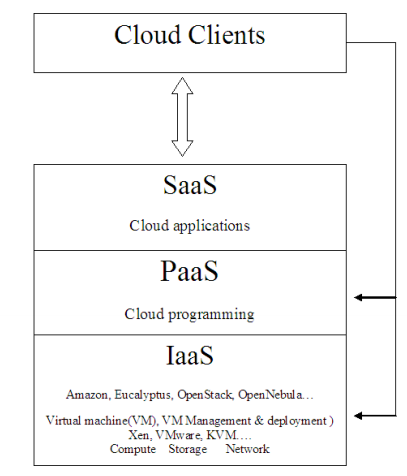
\includegraphics[width=.3\textwidth]{figuras/cloud_structure.png}
\caption{Cloud computing services structure. Cited from: \cite{sefraoui2012openstack}}
\label{fig:cloud_structure}
\end{figure}

% De acordo com Filho e Dionísio \cite{leite2016influencia} (apud \cite{mell2011nist}), os serviços de nuvens devem possuir as seguintes
% características: autoatendimento sob demanda, amplo acesso a rede,
% agrupamento de recursos, elasticidade rápida e medição de serviço.

Accordingly to Filho and Dionísio \cite{leite2016influencia} (apud \cite{mell2011nist}), the cloud services should has the following 
characteristics: self-service on demand, large network access, resource grouping, fast elasticity and service measurement.

% Sefraoui et al. \cite{sefraoui2012openstack} afirmam que a IaaS é onde o recurso de hardware é provido em forma de máquinas vituais. 
% O cliente mantém as aplicações, bancos de dados e servidores enquanto o servidor mantém a virtualização da nuvem, 
% o hardware, o armazenamento e as redes. 

Sefraoui et al. \cite{sefraoui2012openstack} characterize the IaaS as a hardware resource provided on virtual machines. The client
maintains the applications, data bases and servers while the server maintains the cloud virtualization, the hardware, the storage and the networks.   

% Para Bhardwaj et al. \cite{bhardwaj2010cloud}, o modelo IaaS é o serviço de entrega de hardware 
% (servidor, armazenamento e rede) e software associado (sistema de arquivos e virtualização de sistemas). Os autores estabelecem
% os seguintes serviços a serem providos  por IaaS: Infraestrutura virtual (servidor, armazenamento e rede);
% Implantação de aplicativos baseados na Web para fácil disponibilização sob demanda; Balanceamento de carga; 
% Estabelecimento de acordos de nível de serviço com os clientes;  Segurança dos CPUs, dados e rede;
% e Gestão e provisionamento de conta.

To Bhardwaj et al. \cite{bhardwaj2010cloud} the IaaS model is the service of delivering hardware (server, storage and network) 
and associated software (files system and systems virtualization). The authors established the following services to IaaS: 
virtual infraestructure (server, storage and network); Deploy of web-based applications to easy on demand availability;
Load balancer; Establishing service level agreements with the clients; CPUs, data and network security; and Management and 
count provisioning.

% \subsection{Qualidade de Serviço}
\subsection{Quality of Service}

% A qualidade de serviço na computação em nuvem pode ser considerada como o
% desempenho de modo geral do serviço provido \cite{openstack}.

The quality of service in cloud computing can be considered as the performance of service in a general mode \cite{openstack}.

% Filho e Dionísio \cite{leite2016influencia} tratam a qualidade de serviço em duas abordagens:
% uma relacionada à rede e outra em nível de aplicação. Em relação a rede são tratados
% os requisitos para garantir a qualidade do serviço. Em nível de aplicação são tratados
% os atributos que implicam no cumprimento dos níveis de serviço acordado. 

Filho e Dionísio \cite{leite2016influencia} characterize the QoS in two approaches: network and application. In the
network approach deal with the requirements to assure the QoS. The application approach deal with the attributes
that imply on the fulfillment of the service level agreed.

% A qualidade de serviço também pode ser dividida em dois pontos de vista: o 
% ponto de vista do cliente e o ponto de vista do provedor \cite{openstack, bhardwaj2010cloud}. 
% O escopo deste trabalho trata apenas das métricas relacionadas ao ponto de vista do provedor.

The QoS can be divided on two points of view: of the client and of the provider \cite{openstack, bhardwaj2010cloud}. The 
scope of this work deal with metrics only on provider point of view.


\section{OpenStack}

The Openstack is a tool that provides cloud services on IaaS model. Consists in a group of interrelated subprojects that controls a set of processing resources (\textit{Nova} subproject), storage (\textit{Cinder} and \textit{Swift} subprojects), and network (\textit{Neutron} subproject). Each subproject is a module of Openstack and form a computing cloud infrastructure \cite{openstack} \cite{bui2016}.

% O OpenStack é uma ferramenta que fornece serviços de computação em nuvem no modelo IaaS e consiste em um grupo de subprojetos (cada subprojeto é um módulo 
% do OpenStack) inter-relacionados 
% que controlam um conjunto de recursos de processamento (subprojeto \textit{Nova}), armazenamento (subprojetos \textit{Cinder} e \textit{Swift}),
% e de rede (subprojeto \textit{Neutron}) em uma infraestrutura de computação em nuvem \cite{openstack} \cite{bui2016}.

The Openstack provide too some shared services between the different modules, as the authentication and
authorization service (\textit{Keystone} subproject), image service (\textit{Glance} subproject) and the
telemetry service (\textit{Ceilometer} subproject). These are just the mainly services provided by Openstack,
the whole description of all services can be seen in the documentation of the tool \cite{openstack}.

% Além desses subprojetos apresentados, o OpenStack conta com alguns serviços compartilhados entre os diferentes módulos, como o serviço de 
% autenticação e autorização (subprojeto \textit{Keystone}), serviço de gerenciamento de imagens (subprojeto \textit{Glance}) e o serviço de 
% telemetria (subprojeto \textit{Ceilometer}) \cite{openstack}. Estes são apenas os principais serviços providos pelo OpenStack, a
% descrição completa de todos os serviços pode ser vista na documentação da ferramenta \cite{openstack}.

The Openstack is fairly robust. It is capable to control a large number of computional resources
in a datacenter. This characteristic require a good hardware infrastructure for full operation.

% O OpenStack é bastante robusto, capaz de controlar uma grande de quantidade
% de recursos computacionais em um \textit{data center}, o que exige uma infraestrutura de \textit{hardware} 
% considerável para seu funcionamento pleno \cite{openstack_general} \cite{openstack}.

The cloud infrastructure management and control can be realized using a Web application (\textit{Horizon} subproject), via command line (\textit{Command Line Interface} (CLI)) and/or RESTful APIs \cite{bui2016} \cite{openstack}. 

% O gerenciamento e controle da infraestrutura da nuvem pelo usuário podem ser realizados por meio de uma aplicação \textit{Web}
% (subprojeto \textit{Horizon}), via linha de comando (\textit{Command Line Interface} (CLI)) e/ou APIs RESTful \cite{bui2016} \cite{openstack}.

The internal modules integration is realized by RESTful APIs and Remote Procedure Call (RPC) via RabbitMQ
(tool that implements the interprocesses communication following the Advanced Message Queue Protocol) \cite{bui2016}. More details about the modules integration can be seen in the study made by  \cite{bui2016}.

% Em relação à integração interna dos módulos do \textit{OpenStack}, esta é realizada por meio de APIs RESTful e 
% de \textit{Remote Procedure Call} (RPC) via RabbitMQ (ferramenta que implementa a comunicação inter-processos seguindo o protocolo
% \textit{Advanced Message Queue Protocol})\cite{bui2016}. Mais detalhes sobre a integração dos módulos podem ser vistos no estudo de Bui \cite{bui2016}.

The Figure \ref{fig:openstack_architecture} shows the conceptual arquitecture of the Openstack, presenting the relationship between the modules. 
% A Figura \ref{fig:openstack_architecture} ilustra a arquitetura conceitual do OpenStack, apresentando o relacionamento entre os
% módulos que o compõe.

\begin{figure}[ht]
\centering
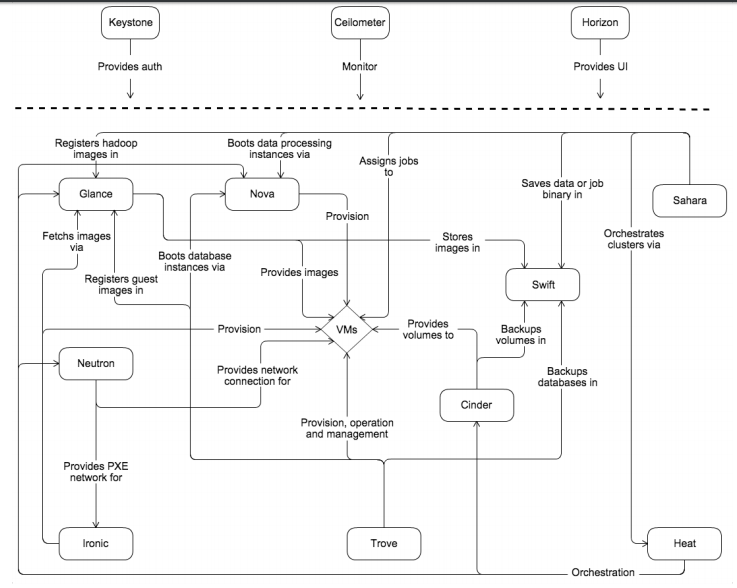
\includegraphics[width=.5\textwidth]{figuras/openstack_architecture.png}
% \caption{Arquitetura conceitual do OpenStack. Fonte: \cite{openstack}}
\caption{Conceptual Arquitecture of the OpenStack. Cited from: \cite{openstack}}
\label{fig:openstack_architecture}
\end{figure}

% \section{Materiais e métodos}
\section{Materials and methods}

The methodology used on this study was organized in five steps that can be seen on Figure \ref{metodologia}.
% Para atingir o objetivo deste trabalho foi utilizada a metodologia apresentada na Figura \ref{metodologia}.

\begin{figure}[ht]
  \centering
  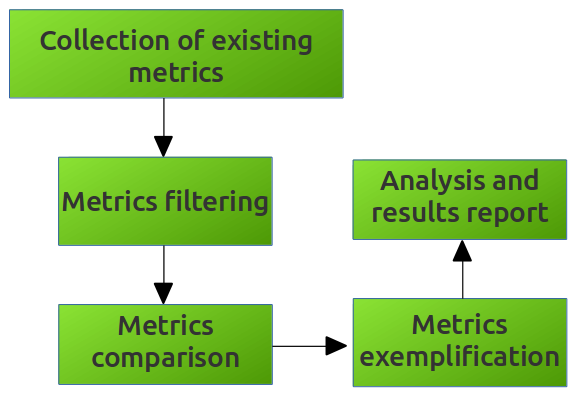
\includegraphics[width=.3\textwidth]{figuras/metodologia.png}
  % \caption{Metodologia proposta. Fonte: Autores.}
  \caption{Proposed methodology.}
  \label{metodologia}
\end{figure}


\begin{itemize}
 % \item \textbf{Levantamento das métricas existentes} - Esta etapa consistiu em consultar na literatura as métricas de QoS para serviços de nuvem e documentá-las, por meio de uma revisão de literatura;
 
 \item \textbf{Collection of existing metrics} - This step consisted in search at literature the QoS metrics to cloud services and document them, using a literature review;

 % \item \textbf{Filtragem das métricas} - A partir das métricas levantadas com a revisão da literatura, esta etapa consistiu em filtrar os resultados a partir de critérios previamente definidos.
  
 \item \textbf{Metrics filtering} - From identified metrics on literature review this step consisted in
 filter the results considering previously defined criterias;


 % \item \textbf{Confronto das métricas} - Esta etapa consistiu em verificar a existência das métricas filtradas no Openstack,	
	% com base na documentação e execução da ferramenta, identificando também como a ferramenta apresenta essa métrica,
	% para verificar quais métricas propostas na literatura são implementadas nativamente no OpenStack. Além disso,
	% métricas que Openstack fornecia mas não se encontravam na literatura, porém estavam relacionadas com as métricas encontradas,
	% foram identificadas e documentadas;

  \item \textbf{Metrics comparison} - For verifying what metrics proposed on literature were natively implemented on Openstack, this step consisted in verify the existence of the filtered metrics on Openstack, based on documentation and tool execution. The form that the tool presents the metrics was identified too. Besides that, the metrics provided by Openstack that was not found on literature, but were related with the found metrics, were identified and documented;
 
 % \item \textbf{Exemplificação das métricas} - Esta etapa consistiu em verificar se as métricas confrontadas constavam realmente na ferramenta e
	% como eram fornecidas,
	% realizando uma simples coleta das métricas idenficadas presentes no Openstack a partir da execução da ferramenta em um cenário de teste.
	% Esta etapa englobou as seguintes atividades:
 \item \textbf{Metrics exemplification} - This step consisted in verify if the compared metrics were in
 the tool and how they are provided. The verification was realized through the simple collection of identified metrics present on the Openstack with the execution of the tool in a test scenario;
 This step also involved the following activities:

	% \subitem - \emph{\textbf{Caracterizar cenário/contexto}}: Nesta atividade descreveu-se o contexto da execução da ferramenta e o cenário de teste utilizado,
	% 	 considerando itens como ambiente para execução do teste, versão da ferramenta utilizada, topologia utilizada, ferramentas
	% 	 e recursos disponíveis;
	% \subitem - \emph{\textbf{Coletar dados}}: Nesta atividade as métricas identificadas na etapa anterior foram coletadas e documentadas;

  \subitem - \emph{\textbf{Characterize scenario/context}}: In this activity was described the context of the execution and the test scenario. The scenario was described considering items as the environment for
  the execution, tool version, topology and available tools and resources.

  \subitem - \emph{\textbf{Collect data}}: In this activity the identified metrics on 
  the previous step were collected and documented.

 % \item \textbf{Análise e redação dos resultados}: Nesta etapa os resultados obtidos na etapa anterior foram interpretados e documentados.
 \item \textbf{Analysis and results report}: In this step the obtained results on previous step were
 interpreted and documented.
 
\end{itemize}

\section{Execution} % MELHORAR ESSE TITULO

  \subsection{Collection of existing metrics}
     
%       Foi realizada uma revisão de literatura com o intuito de encontrar as métricas de QoS existentes
%       propostas em outros estudos. Foram encontrados seis artigos que apresentavam de forma explícita métricas de QoS para
%       serviços de nuvem.  Estes artigos foram analisados e foram identificadas 68 métricas que podem ser vistas na Tabela \ref{tab:metricas_literatura}.
      
      A literature review was performed in order to find existing QoS metrics proposed in other studies.
      Six papers that explicitly presented QoS metrics for cloud services were found. These papers were analyzed and then 
      68 metrics were identified, which can be seen in the Table \ref{tab:metricas_literatura}. The found papers are:
      
      \begin{itemize}
       \item \textbf{Paper 1}: \textit{QoS Metrics for Cloud Computing Services Evaluation} \cite{bardsiri2014};
       \item \textbf{Paper 2}: \textit{On a Catalogue of Metrics for Evaluating Commercial Cloud Services} \cite{li2012};
       \item \textbf{Paper 3}: \textit{IaaS Cloud Service Selection using Case-Based Reasoning} \cite{soltani2016};
       \item \textbf{Paper 4}: \textit{SMICloud: A Framework for Comparing and Ranking Cloud Services} \cite{garg2011};
       \item \textbf{Paper 5}: \textit{Cloud Services Measures for Global Use} \cite{siegel2012cloud}
       \item \textbf{Paper 6}: \textit{An End-To-End QoS Mapping Approach for Cloud Service Selection} \cite{karim2013}
      \end{itemize}
      
\begin{table}[]
\centering
 \caption{Metrics found in the literature}
\label{tab:metricas_literatura}
\begin{tabular}{|l|l|l|}
\hline
\multicolumn{1}{|c|}{\textbf{Metric}}                                                       & \multicolumn{1}{c|}{\textbf{Category}}                                                                    & \multicolumn{1}{c|}{\textbf{Paper}}                                                    \\ \hline
Cryptography algorithms                                                                   & Security                                                                                                  & \multirow{9}{*}{Paper 6 [19]}                                                          \\ \cline{1-2}
Service learnability                                                                  & Usability                                                                                                &                                                                                         \\ \cline{1-2}
Access Control                                                                           & Security                                                                                                  &                                                                                         \\ \cline{1-2}
Data Control                                                                            & Data Control                                                                                          &                                                                                         \\ \cline{1-2}
Defects per million (DPM)                                                                    & -                                                                                                          &                                                                                         \\ \cline{1-2}
Ease of use                                                                            & Usability                                                                                                &                                                                                         \\ \cline{1-2}
IaaS instalability                                                                      & Usability                                                                                                &                                                                                         \\ \cline{1-2}
Data Privacy                                                                        & Security                                                                                                  &                                                                                         \\ \cline{1-2}
\begin{tabular}[c]{@{}l@{}}Mean time between \\ failures (MTBF)\end{tabular}                   & Reliability                                                                                             &                                                                                         \\ \hline
Access Control Policies                                                              & \begin{tabular}[c]{@{}l@{}}Security/ \\ Privacy\end{tabular}                                          & Paper 5 [18]                                                                           \\ \hline
VM Cost                                                                                  & Cost                                                                                                      & \begin{tabular}[c]{@{}l@{}}Paper 5 [18] \\ Paper 4 [1]\end{tabular}                  \\ \hline
Storage (HD)         & -                                                                                                          & \multirow{16}{*}{Paper 3 [3]}                                                          \\ \cline{1-2}
NoSQL databases support                                                                         & -                                                                                                          &                                                                                         \\ \cline{1-2}
Application layers                                                                         & -                                                                                                          &                                                                                         \\ \cline{1-2}
CPU frequency                                                                            & -                                                                                                          &                                                                                         \\ \cline{1-2}
I/O performance                                                                           & -                                                                                                          &                                                                                         \\ \cline{1-2}
\begin{tabular}[c]{@{}l@{}}Bandwidth \\ (download, upload)\end{tabular}               & -                                                                                                          &                                                                                         \\ \cline{1-2}
Application maximum latency                                                                  & -                                                                                                          &                                                                                         \\ \cline{1-2}
Number of load balancers                                                             & -                                                                                                          &                                                                                         \\ \cline{1-2}
Number of instances                                                                         & -                                                                                                          &                                                                                         \\ \cline{1-2}
Number of CPU cores                                                                     & -                                                                                                          &                                                                                         \\ \cline{1-2}
\begin{tabular}[c]{@{}l@{}}Concurrent users \\ maximum number\end{tabular}            & -                                                                                                          &                                                                                         \\ \cline{1-2}
Region                                                                                       & -                                                                                                          &                                                                                         \\ \cline{1-2}
Application servers                                                                      & -                                                                                                          &                                                                                         \\ \cline{1-2}
\begin{tabular}[c]{@{}l@{}}Operational System \\ (Type, Platform, Version)\end{tabular}    & -                                                                                                          &                                                                                         \\ \cline{1-2}
Relational database support                                                                    & -                                                                                                          &                                                                                         \\ \cline{1-2}
Application type                                                                            & -                                                                                                          &                                                                                         \\ \hline
Security (general metric)                                                                    & -                                                                                                          & \begin{tabular}[c]{@{}l@{}}Paper 3 [3] \\ Paper 6 [19]\end{tabular}                  \\ \hline
\begin{tabular}[c]{@{}l@{}}Memory (RAM required \\ for the instance)\end{tabular}            & \begin{tabular}[c]{@{}l@{}}Reliability/ \\ Sustainability\end{tabular}                        & \multirow{2}{*}{\begin{tabular}[c]{@{}l@{}}Paper 3 [3] \\ Paper 4 [1]\end{tabular}}  \\ \cline{1-2}
Application response time                                                                & Performance                                                                                                &                                                                                         \\ \hline
Availability                                                                              & -                                                                                                          & \begin{tabular}[c]{@{}l@{}}Paper 3 [3] \\ Paper 4 [1] \\ Paper 6 [19]\end{tabular} \\ \hline
\begin{tabular}[c]{@{}l@{}}Transfer latency \\ TCP/UDP/IP\end{tabular}                & \begin{tabular}[c]{@{}l@{}}Performance / \\ Communication\end{tabular}                          & \multirow{2}{*}{Paper 2 [4]}                                                           \\ \cline{1-2}
\begin{tabular}[c]{@{}l@{}}Transfer speed \\ bit/byte TCP/UDP/IP\end{tabular}   & \begin{tabular}[c]{@{}l@{}}Performance / \\ Communication\end{tabular} &                                                                                         \\ \hline
Confidentiality                                                                            & \begin{tabular}[c]{@{}l@{}}Security /\\ Authentication\end{tabular}                                         & \multirow{9}{*}{Paper 1 [5]}                                                           \\ \cline{1-2}
Effectiveness                                                                                  & \begin{tabular}[c]{@{}l@{}}Security / \\ Authentication\end{tabular}                                        &                                                                                         \\ \cline{1-2}
Auditability                                                                      & \begin{tabular}[c]{@{}l@{}}Security / \\ Data Security\end{tabular}                                 &                                                                                         \\ \cline{1-2}
Modularity                                                                                 & -                                                                                                          &                                                                                         \\ \cline{1-2}
Sensitivity                                                                                & \begin{tabular}[c]{@{}l@{}}Security / \\ Authentication\end{tabular}                                        &                                                                                         \\ \cline{1-2}
Boot time                                                                                & \begin{tabular}[c]{@{}l@{}}Economy / \\ Elasticity\end{tabular}                                         &                                                                                         \\ \cline{1-2}
Computation time                                                                          & \begin{tabular}[c]{@{}l@{}}Performance \end{tabular}                                             &                                                                                         \\ \cline{1-2}
Resources utilization                                                                       & Eficiency                                                                                                 &                                                                                         \\ \cline{1-2}
Memory speed                                                                        & \begin{tabular}[c]{@{}l@{}}Performance /\\  Memória\end{tabular}                                           &                                                                                         \\ \hline
\end{tabular}
\end{table}

\begin{table}
\begin{tabular}{|l|l|l|}
\hline
CPU load                                                                                 & \begin{tabular}[c]{@{}l@{}}Performance /\\ Computação\end{tabular}                                         & \multirow{21}{*}{\begin{tabular}[c]{@{}l@{}}Paper 1 [5] \\ Paper 2 [4]\end{tabular}} \\ \cline{1-2}
\begin{tabular}[c]{@{}l@{}}Component \\ resources cost\end{tabular}                  & Economy / Cost                                                                                           &                                                                                         \\ \cline{1-2}
FLOP cost                                                                               & Economy / Cost                                                                                           &                                                                                         \\ \cline{1-2}
Fixed time cost                                                                         & Economy / Cost                                                                                           &                                                                                         \\ \cline{1-2}
Total cost                                                                                  & Economy / Cost                                                                                           &                                                                                         \\ \cline{1-2}
Instance efficiency                                                                      & \begin{tabular}[c]{@{}l@{}}Performance / \\ Computation\end{tabular}                                        &                                                                                         \\ \cline{1-2}
Packet loss frequency                                                               & \begin{tabular}[c]{@{}l@{}}Performance / \\ Communication\end{tabular}                                       &                                                                                         \\ \cline{1-2}
\begin{tabular}[c]{@{}l@{}}Latency over SLL\end{tabular}                 & \begin{tabular}[c]{@{}l@{}}Security / \\ Data Security\end{tabular}                                 &                                                                                         \\ \cline{1-2}
Price/Performance ratio                                                                      & Economy / Cost                                                                                           &                                                                                         \\ \cline{1-2}
Is SSL applicable?                                                                               & \begin{tabular}[c]{@{}l@{}}Security / \\ Data Security\end{tabular}                                 &                                                                                         \\ \cline{1-2}
RAM update rate                                                                   & \begin{tabular}[c]{@{}l@{}}Performance / \\ Memory\end{tabular}                                           &                                                                                         \\ \cline{1-2}
Connection errors rate                                                                     & \begin{tabular}[c]{@{}l@{}}Performance / \\ Communication\end{tabular}                                       &                                                                                         \\ \cline{1-2}
\begin{tabular}[c]{@{}l@{}}FLOPs (Float Point Operations \\ Per Second) rate\end{tabular} & \begin{tabular}[c]{@{}l@{}}Performance / \\ Computation\end{tabular}                                        &                                                                                         \\ \cline{1-2}
Communication time                                                                         & Performance                                                                                        &                                                                                         \\ \cline{1-2}
Deletion time                                                                             & \begin{tabular}[c]{@{}l@{}}Economy / \\ Elasticity\end{tabular}                                          &                                                                                         \\ \cline{1-2}
Deploy time                                                                         & \begin{tabular}[c]{@{}l@{}}Economy / \\ Elasticity\end{tabular}                                         &                                                                                         \\ \cline{1-2}
Suspension time                                                                           & \begin{tabular}[c]{@{}l@{}}Economy / \\ Elasticity\end{tabular}                                         &                                                                                         \\ \cline{1-2}
Acquisition total time                                                                     & \begin{tabular}[c]{@{}l@{}}Economy / \\ Elasticity\end{tabular}                                         &                                                                                         \\ \cline{1-2}
\begin{tabular}[c]{@{}l@{}}Supported Users on \\ a Fixed Budget\end{tabular}          & Economy / Cost                                                                                           &                                                                                         \\ \cline{1-2}
Interoperability                                                                           & -                                                                                                          &                                                                                         \\ \cline{1-2}
Memory reponse time                                                                   & \begin{tabular}[c]{@{}l@{}}Performance / \\ Memory\end{tabular}                                           &                                                                                         \\ \hline
Accuracy                                                                                     & -                                                                                                          & \multirow{5}{*}{Paper 4 [1]}                                                           \\ \cline{1-2}
Adequacy                                                                                    & -                                                                                                          &                                                                                         \\ \cline{1-2}
Reliability (errors numbers)                                                                               & -                                                                                                          &                                                                                         \\ \cline{1-2}
Elasticity                                                                                 & -                                                                                                          &                                                                                         \\ \cline{1-2}
Transparency                                                                                & -                                                                                                          &                                                                                         \\ \hline
\end{tabular}
\end{table}

     
  \subsection{Metrics filtering}
  
%       Para a filtragem das métricas foram definidos quatro critérios considerando o contexto e escopo do trabalho. A avaliação das
%       métricas coletadas pode ser vista na Tabela \ref{tab:avaliacao_metricas}.
	
	Four criteria were defined to filter the metrics considering the context and scope of the work.
	The evaluation of the collected metrics can be seen in Table \ref{tab:avaliacao_metricas}.
   
	\begin{itemize}
% 	 \item \textbf{Critério 1 - O significado é conhecido?}
	 \item \textbf{Criterion 1 - Is the meaning known?}
% 	    \subitem Esse critério foi utilizado para avaliar se o significado da métrica e sua forma de cálculo eram conhecidos.
	    \subitem This criterion was used to assess if the meaning of the metric and its calculation method were known.
	    
% 	 \item \textbf{Critério 2 - Aplica-se para o modelo de serviço IaaS?}
	 \item \textbf{Criterion 2 - Does it apply to the IaaS service model?}
% 	    \subitem Este critério foi utilizado para selecionar as métricas propícias ao modelo IaaS, devido às suas características peculiares;
	    \subitem This criterion was used to select the propitious metrics to IaaS model, due to its singular characteristics.
	    
% 	 \item \textbf{Critério 3 - Pode ser coletada objetivamente?}
	 \item \textbf{Criterion 3 - Can it be collected objectively?}
% 	    \subitem Este critério foi utilizado para selecionar as métricas que são coletadas de forma objetiva, pois este tipo
% 	    de métrica pode ser coletado por meio de ferramentas;
	    \subitem This criterion was used to select the metrics that can be collected objectively, because this kind of metric
	    can be collected using automated tools.
	    
% 	 \item \textbf{Critério 4 - É do ponto de vista do provedor?}
	 \item \textbf{Criterion 4 - Is it from the provider's perspective?}
% 	    \subitem Este critério foi utilizado para selecionar as métricas que se tratavam do ponto de vista do provedor do serviço de nuvem;
	    \subitem This criterion was used to select which metrics were related to the cloud computing service provider point of view.
	\end{itemize}

\begin{table*}[]
\centering
% \caption{Avaliação das métricas nos critérios definidos}
\caption{Metrics evaluation according to defined criteria}
\label{tab:avaliacao_metricas}
\begin{tabular}{@{}lcccc@{}}
\toprule
\multicolumn{1}{c}{\textbf{Metric}}              & \multicolumn{1}{l}{\textbf{Criteria 1}} & \multicolumn{1}{l}{\textbf{Criteria 2}} & \multicolumn{1}{l}{\textbf{Criteria 3}} & \textbf{Criteria 4}         \\ \midrule
Transfer latency TCP/UDP/IP                & Yes                                     & Yes                                     & Yes                                     & Yes                         \\
Bandwidth (download, upload)               & Yes                                     & Yes                                     & Yes                                     & Yes                         \\
CPU load                                      & Yes                                     & Yes                                     & Yes                                     & Yes                         \\
Reliability (errors numbers)                  & Yes                                     & Yes                                     & Yes                                     & Yes                         \\
Access Control                                & Yes                                     & Yes                                     & Yes                                     & Yes                         \\
CPU frequency                                 & Yes                                     & Yes                                     & Yes                                     & Yes                         \\
Total cost                                       & Yes                                     & Yes                                     & Yes                                     & Yes                         \\
Instance efficiency                           & Yes                                     & Yes                                     & Yes                                     & Yes                         \\
Elasticity                                      & Yes                                     & Yes                                     & Yes                                     & Yes                         \\
Packet loss frequency                    & Yes                                     & Yes                                     & Yes                                     & Yes                         \\
Auditability                           & Yes                                     & Yes                                     & Yes                                     & Yes                         \\
Latency over SLL                 & Yes                                     & Yes                                     & Yes                                     & Yes                         \\
Application maximum latency                       & Yes                                     & Yes                                     & Yes                                     & Yes                         \\
Concurrent users maximum number            & Yes                                     & Yes                                     & Yes                                     & Yes                         \\
Memory (RAM required for the instance)            & Yes                                     & Yes                                     & Yes                                     & Yes                         \\
NoSQL databases support                    & Yes                                     & Yes                                     & Yes                                     & Yes                         \\
Number of CPU cores                          & Yes                                     & Yes                                     & Yes                                     & Yes                         \\
Number of instances                               & Yes                                     & Yes                                     & Yes                                     & Yes                         \\
Number of load balancers                  & Yes                                     & Yes                                     & Yes                                     & Yes                         \\
Operational System (Type, Platform, Version)    & Yes                                     & Yes                                     & Yes                                     & Yes                         \\
Relational database support                         & Yes                                     & Yes                                     & Yes                                     & Yes                         \\
Memory reponse time                        & Yes                                     & Yes                                     & Yes                                     & Yes                         \\
Is SSL applicable?                                    & Yes                                     & Yes                                     & Yes                                     & Yes                         \\
Storage (HD)        & Yes                                     & Yes                                     & Yes                                     & Yes                         \\
Boot time                                     & Yes                                     & Yes                                     & Yes                                     & Yes                         \\
Communication time                              & Yes                                     & Yes                                     & Yes                                     & Yes                         \\
Deletion time                                  & Yes                                     & Yes                                     & Yes                                     & Yes                         \\
Deploy time                              & Yes                                     & Yes                                     & Yes                                     & Yes                         \\
Application response time                     & Yes                                     & Yes                                     & Yes                                     & Yes                         \\
Suspension time                                & Yes                                     & Yes                                     & Yes                                     & Yes                         \\
Mean time between failures (MTBF)                   & Yes                                     & Yes                                     & Yes                                     & Yes                         \\
Acquisition total time                          & Yes                                     & Yes                                     & Yes                                     & Yes                         \\
Transfer speed bit/byte TCP/UDP/IP   & Yes                                     & Yes                                     & Yes                                     & Yes                         \\
I/O performance                                & Yes                                     & Yes                                     & Yes                                     & Yes                         \\
Accuracy                                          & Yes                                     & Yes                                     & Yes                                     & \cellcolor[HTML]{EA9999}No \\
Availability                                   & Yes                                     & Yes                                     & Yes                                     & \cellcolor[HTML]{EA9999}No \\
Adequacy                                         & Yes                                     & \cellcolor[HTML]{EA9999}No             & \cellcolor[HTML]{EA9999}-               & \cellcolor[HTML]{EA9999}-   \\
Service learnability                       & Yes                                     & Yes                                     & \cellcolor[HTML]{EA9999}No             & \cellcolor[HTML]{EA9999}-   \\
Data Control                                 & Yes                                     & Yes                                     & \cellcolor[HTML]{EA9999}No             & \cellcolor[HTML]{EA9999}-   \\
Fixed time cost                              & Yes                                     & Yes                                     & \cellcolor[HTML]{EA9999}No             & \cellcolor[HTML]{EA9999}-   \\
Defects per million                               & Yes                                     & \cellcolor[HTML]{EA9999}No             & \cellcolor[HTML]{EA9999}-               & \cellcolor[HTML]{EA9999}-   \\
Ease of use                                 & Yes                                     & Yes                                     & \cellcolor[HTML]{EA9999}No             & \cellcolor[HTML]{EA9999}-   \\
IaaS instalability                           & Yes                                     & Yes                                     & \cellcolor[HTML]{EA9999}No             & \cellcolor[HTML]{EA9999}-   \\
Interoperability                                & Yes                                     & Yes                                     & \cellcolor[HTML]{EA9999}No             & \cellcolor[HTML]{EA9999}-   \\
Access Control Policies                   & Yes                                     & Yes                                     & \cellcolor[HTML]{EA9999}No             & \cellcolor[HTML]{EA9999}-   \\
Transparency                                     & Yes                                     & Yes                                     & \cellcolor[HTML]{EA9999}No             & \cellcolor[HTML]{EA9999}-   \\
VM Cost                                       & Yes                                     & Yes                                     & \cellcolor[HTML]{EA9999}No             & \cellcolor[HTML]{EA9999}-   \\
Cryptography algorithms                        & \cellcolor[HTML]{EA9999}No             & \cellcolor[HTML]{EA9999}-               & \cellcolor[HTML]{EA9999}-               & \cellcolor[HTML]{EA9999}-   \\
Application servers                           & \cellcolor[HTML]{EA9999}No             & \cellcolor[HTML]{EA9999}-               & \cellcolor[HTML]{EA9999}-               & \cellcolor[HTML]{EA9999}-   \\
Application layers                              & \cellcolor[HTML]{EA9999}No             & \cellcolor[HTML]{EA9999}-               & \cellcolor[HTML]{EA9999}-               & \cellcolor[HTML]{EA9999}-   \\
Application type                                 & \cellcolor[HTML]{EA9999}No             & \cellcolor[HTML]{EA9999}-               & \cellcolor[HTML]{EA9999}-               & \cellcolor[HTML]{EA9999}-   \\
Confidentiality                                 & \cellcolor[HTML]{EA9999}No             & \cellcolor[HTML]{EA9999}-               & \cellcolor[HTML]{EA9999}-               & \cellcolor[HTML]{EA9999}-   \\
Component resources cost                  & \cellcolor[HTML]{EA9999}No             & \cellcolor[HTML]{EA9999}-               & \cellcolor[HTML]{EA9999}-               & \cellcolor[HTML]{EA9999}-   \\
FLOP cost                                    & \cellcolor[HTML]{EA9999}No             & \cellcolor[HTML]{EA9999}-               & \cellcolor[HTML]{EA9999}-               & \cellcolor[HTML]{EA9999}-   \\
Effectiveness                                       & \cellcolor[HTML]{EA9999}No             & \cellcolor[HTML]{EA9999}-               & \cellcolor[HTML]{EA9999}-               & \cellcolor[HTML]{EA9999}-   \\
Modularity                                      & \cellcolor[HTML]{EA9999}No             & \cellcolor[HTML]{EA9999}-               & \cellcolor[HTML]{EA9999}-               & \cellcolor[HTML]{EA9999}-   \\
Data privacy                             & \cellcolor[HTML]{EA9999}No             & \cellcolor[HTML]{EA9999}-               & \cellcolor[HTML]{EA9999}-               & \cellcolor[HTML]{EA9999}-   \\
Price/Performance ratio                           & \cellcolor[HTML]{EA9999}No             & \cellcolor[HTML]{EA9999}-               & \cellcolor[HTML]{EA9999}-               & \cellcolor[HTML]{EA9999}-   \\
Region                                            & \cellcolor[HTML]{EA9999}No             & \cellcolor[HTML]{EA9999}-               & \cellcolor[HTML]{EA9999}-               & \cellcolor[HTML]{EA9999}-   \\
Security (general metric)                         & \cellcolor[HTML]{EA9999}No             & \cellcolor[HTML]{EA9999}-               & \cellcolor[HTML]{EA9999}-               & \cellcolor[HTML]{EA9999}-   \\
Sensitivity                                     & \cellcolor[HTML]{EA9999}No             & \cellcolor[HTML]{EA9999}-               & \cellcolor[HTML]{EA9999}-               & \cellcolor[HTML]{EA9999}-   \\
RAM update rate                        & \cellcolor[HTML]{EA9999}No             & \cellcolor[HTML]{EA9999}-               & \cellcolor[HTML]{EA9999}-               & \cellcolor[HTML]{EA9999}-   \\
FLOPs (Float Point Operations Per Second) rate & \cellcolor[HTML]{EA9999}No             & \cellcolor[HTML]{EA9999}-               & \cellcolor[HTML]{EA9999}-               & \cellcolor[HTML]{EA9999}-   \\
Computation time                               & \cellcolor[HTML]{EA9999}No             & \cellcolor[HTML]{EA9999}-               & \cellcolor[HTML]{EA9999}-               & \cellcolor[HTML]{EA9999}-   \\
Supported Users on a Fixed Budget          & \cellcolor[HTML]{EA9999}No             & \cellcolor[HTML]{EA9999}-               & \cellcolor[HTML]{EA9999}-               & \cellcolor[HTML]{EA9999}-   \\
Resources utilization                            & \cellcolor[HTML]{EA9999}No             & \cellcolor[HTML]{EA9999}-               & \cellcolor[HTML]{EA9999}-               & \cellcolor[HTML]{EA9999}-   \\
Memory speed                             & \cellcolor[HTML]{EA9999}No             & \cellcolor[HTML]{EA9999}-               & \cellcolor[HTML]{EA9999}-               & \cellcolor[HTML]{EA9999}-   \\
Connection errors rate                          & \cellcolor[HTML]{EA9999}No             & \cellcolor[HTML]{EA9999}-               & \cellcolor[HTML]{EA9999}-               & \cellcolor[HTML]{EA9999}-   \\ \bottomrule
\end{tabular}
\end{table*}
   
  \subsection{Metrics comparison} \label{confronto}
  
  % Com a filtragem obteve-se 34 métricas resultantes a serem confrontadas no Openstack. Para isso, as métricas foram divididas em estáticas e
  % dinâmicas, ou seja, aquelas que não necessitam de execução da ferramenta para serem coletadas e aquelas que necessitam da execução da ferramenta,
  % respectivamente. Além disso, as métricas foram categorizadas com base no estudo de Bardsiri e Hashemi \cite{bardsiri2014}.As categorias foram:
  % Confiabilidade, Economia, Memória, Performance, Segurança e Geral. Vale ressaltar, que foram identificadas duas métricas equivalentes (Velocidade de transferência bit/byte TCP/UDP/IP
  % e Largura de Banda (download, upload)) e dessa forma, apenas a Largura de Banda foi considerada na avaliação.
  
  After the filtering step it was obtained 34 resulting metrics to be compared on the Openstack. For making this, the metrics were organized in static metrics and dynamic metrics. The static metrics do not need of tool execution to be collected while the dynamic metrics have this necessity. Besides that, the metrics were categorized based on the study realized by Bardsiri e Hashemi \cite{bardsiri2014}. 

  The used categories were: Reliability, Economy, Memory, Performance,
  Security and General. It is worth mentioning that were identified two equivalent metrics: Transfer Speed bit/byte TCP/UDP/IP and Bandwidth (download, upload). Considering this, only bandwidth was used on comparison.

 %  A categorização e o confronto das métricas pode ser visualizado nas Tabelas   \ref{tab:confronto_estaticas} e \ref{tab:confronto_dinamicas}  
 % que representam as métricas estáticas e dinâmicas, respectivamente. 

  The categorization and the metrics comparison is presented on Tables \ref{tab:confronto_estaticas} and \ref{tab:confronto_dinamicas} that represents the static metrics and dynamic metrics, respectively.

\begin{table}[ht]
\centering
% \caption{Avaliação das métricas estáticas existentes no Openstack}
\caption{Static metrics evaluation on Openstack}
\label{tab:confronto_estaticas}
\begin{tabular}{@{}lll@{}}
\toprule
\multicolumn{3}{c}{\textbf{Statics}}                                                                  \\ \midrule
\multicolumn{1}{c}{\textbf{Category}} & \multicolumn{1}{c}{\textbf{Metrics}}                                                  & \multicolumn{1}{c}{\textbf{Is it provided by the Openstack?}} \\
Economy                   & Total cost                                    & -                         \\
\multirow{3}{*}{General}     & NoSQL databases support                 & Yes                       \\
                           & \begin{tabular}[c]{@{}l@{}}Operational System \\ (Type, Platform, Version)\end{tabular} & Yes                       \\
                           & Relational database support                 & Yes                       \\
\multirow{3}{*}{Security} & Access control policies                             & Yes                       \\
                           & Is SSL applicable?                             & Yes                       \\
                           & Auditability                        & Yes                       \\ \bottomrule
\end{tabular}
\end{table}  

\begin{table}[ht]
\centering
% \caption{Avaliação das métricas dinâmicas existentes no Openstack}
\caption{Dynamic metrics evaluation on Openstack}
\label{tab:confronto_dinamicas}
\begin{tabular}{@{}lll@{}}
\toprule
\multicolumn{3}{c}{\textbf{Dynamics}}                                                                  \\ \midrule
\multicolumn{1}{c}{\textbf{Category}} & \multicolumn{1}{c}{\textbf{Metrics}}                                                  & \multicolumn{1}{c}{\textbf{Is it provided by the Openstack?}} \\
\multirow{2}{*}{Reliability}        & Reliability (errors numbers)                                                      & No                                           \\
                                       & Mean time between
failures (MTBF)                                                       & No                                           \\
\multirow{6}{*}{Economy}              & Elasticity                                                                          & No                                           \\
                                       & Boot time                                                                         & No                                           \\
                                       & Deletion time                                                                      & No                                           \\
                                       & Deploy time                                                                  & No                                           \\
                                       & Suspension Time                                                                    & No                                           \\
                                       & Acquisition total time                                                              & No                                           \\
\multirow{2}{*}{Memory}               & \begin{tabular}[c]{@{}l@{}}Memory (RAM required \\ for the instance)\end{tabular}     & Yes                                           \\
                                       & \begin{tabular}[c]{@{}l@{}}Storage (HD)\end{tabular} & Yes                                           \\
\multirow{15}{*}{Performance}          & Application maximum latency -                                                          & No                                           \\
                                       & \begin{tabular}[c]{@{}l@{}}Concurrent users \\ maximum number\end{tabular}     & No                                           \\
                                       & Number of CPU cores                                                               & No                                           \\
                                       & Number of instances                                                                  & Yes                                           \\
                                       & Number of load balancers                                                     & No                                           \\
                                       & Application response time                                                         & No                                           \\
                                       & Bandwidth (download, upload)                                                   & Yes                                           \\
                                       & CPU load                                                                          & Yes                                           \\
                                       & CPU frequency                                                                     & Yes                                           \\
                                       & Instance efficiency                                                               & Yes                                           \\
                                       & Packet loss frequency                                                        & No                                           \\
                                       & Transfer latency TCP/UDP/IP                                                    & No                                           \\
                                       & I/O Performance                                                                    & Yes                                           \\
                                       & Memory reponse time                                                           & No                                           \\
                                       & Communication time                                                                  & No                                           \\
Security                              & Latency over SLL                                                     & No                                           \\ \bottomrule
\end{tabular}
\end{table}  

% As métricas existentes no Openstack podem ser sumarizadas nos itens abaixo.
% Além das métricas idênticas ao que foi levantado, foram identificadas outras
% métricas relacionadas. Todas as métricas fornecidas pela ferramenta podem ser consultadas na documentação \cite{openstack}.

The existent metrics on the Openstack can be sumarized in the following items. Beyond of the identical metrics, related metrics were identified.
All metrics provided by the tool can be consulted in the documentation \cite{openstack}.

\begin{itemize}
 \item \textbf{Memory (RAM required for the instance)}
    \subitem - Volume of RAM allocated to the instance (memory);
    \subitem - Volume of RAM used by the instance from the amount of its allocated memory (memory.usage);
    \subitem - Volume of RAM used per project.
 \item \textbf{Storage (HD)}
    \subitem - Size of root disk (disk.root.size);
    \subitem - Permanent memory used per project;
 \item \textbf{Application maximum latency}
    \subitem - Average disk latency (disk.latency);
    \subitem - Average disk latency per device (disk.device.latency).
 \item \textbf{Number of CPU cores}
    \subitem - Number of virtual CPUs allocated to the instance (vcpus);
    \subitem - Number of virtual CPUs per project;
    \subitem - Average CPU utilization (cpu\_util).
 \item \textbf{Number of instances}
    \subitem - Number of active instances.
 \item \textbf{Number of load balancers}
  \subitem - Existence of a LB pool (network.services.lb.pool)
  \subitem - Existence of a LB VIP (network.services.lb.vip )
  \subitem - Existence of a LB member (network.services.lb.member)
  \subitem - Existence of a LB health probe (network.services.lb.health\_monitor)
  \subitem - Total connections on a LB (network.services.lb.total.connections)
  \subitem - Active connections on a LB (network.services.lb.active.connections)
  \item \textbf{Bandwidth (download, upload)}
    \subitem - Bytes through this l3 metering label (Network layer routers) (bandwidth).
  \item \textbf{CPU load}   
    \subitem - CPU load in the past 1 minute (hardware.cpu.load.1min);
    \subitem - CPU load in the past 5 minutes (hardware.cpu.load.5min);
    \subitem - CPU load in the past 10 minutes (hardware.cpu.load.10min);
  \item \textbf{CPU frequency}  
    \subitem - CPU frequency (compute.node.cpu.frequency);
  \item \textbf{Instance efficiency}    
    \subitem - CPU utilization (compute.node.cpu.percent);
  \item \textbf{Packet loss frequency}   
    \subitem - Number of incoming packets (network.incoming.packets)
    \subitem - Average rate of incoming packets (network.incoming.packets.rate)
    \subitem - Number of outgoing packets (network.outgoing.packets)
    \subitem - Average rate of outgoing packets (network.outgoing.packets.rate)
  \item \textbf{I/O Performance} 
    \subitem - Number of read requests (disk.read.requests)
    \subitem - Average rate of read requests (disk.read.requests.rate)
    \subitem - Number of write requests (disk.write.requests)
    \subitem - Average rate of write requests (disk.write.requests.rate)
    \subitem - Volume of reads (disk.read.bytes)
    \subitem - Average rate of reads (disk.read.bytes.rate)
    \subitem - Volume of writes (disk.write.bytes)
    \subitem - Average rate of writes (disk.write.bytes.rate)
 \end{itemize}  

  \subsection{Metrics exemplification} 
%     Para verificar como se apresentavam as métricas ditas presentes no OpenStack, foi executado um cenário de teste de uso da ferramenta
%     para coletar tais métricas obtidas na seção \ref{confronto}. 
%     A Subseção \ref{cenario} descreve o cenário utilizado e a Subseção \ref{resultados_levantamento} discorre sobre os resultados obtidos.

      In order to verify how the presented metrics were presented in OpenStack, a tool usage test scenario was performed to collect
      such metrics obtained in section \ref{confronto}.
      The Subsection \ref{cenario} describes the used scenario and the Subsection \ref{resultados_levantamento} discusses the obtained results.
  
    \subsubsection{\textbf{Test scenario}} \label{cenario}
	
% 	A coleta dos dados foi realizada no seguinte cenário/contexto:
	The data collection was performed in the following scenario/context: 
	
% 	\begin{itemize}
% % 	 \item Duas pessoas com dedicação parcial como equipe de coleta ; % COLOCA DEDICAÇÃO PARCIAL ?
% 	 \item Laboratório com máquinas que possuiam recursos de \textit{hardware} simples;
% 	    \subitem Apenas máquinas com 4GB de memória RAM no máximo.
% 	 \item Utilização da versão \textit{Kilo} do OpenStack;
% 	 \item Utilização do CentOS 7 \cite{centos} como sistema operacional;
% 	 \item Utilização da topologia apresentada na Figura \ref{fig:topologia} para instalação do OpenStack;
% 	    \subitem Foram utilizados dois computadores interconectados para distribuir a carga de processamento entre eles, 
% 		  de modo que um computador ficava com o nó Controlador (\textit{Controller}) e o outro computador ficava
% 		     com os nós de Processamento (\textit{Compute}) e de Rede (\textit{Network}), como ilustra a Figura \ref{fig:topologia};
% 	    \subitem A topologia utilizada foi baseada na topologia proposta por Ahmad Imanudin em \cite{imanudin};
% 	  \item Criação de duas instâncias.
% 	\end{itemize}
	
	\begin{itemize}
	 \item Laboratory with machines that had simple hardware features;
	    \subitem Only machines with 4GB of RAM at most.
	 \item Use of OpenStack Kilo version;
	 \item Use of CentOS 7 \cite{centos} as operational system;
	 \item Use of the topology presented in Figure \ref{fig:topologia} to OpenStack installation;
	    \subitem Two interconnected computers were used to distribute the processing load between them,
		     so that a computer had the Controller node and the other computer had the Processing (Compute) and the Network
		     nodes as shown in Figure \ref{fig:topologia};
	    \subitem The topology used was based on the topology proposed by Ahmad Imanudin in \cite{imanudin};
	  \item Creation of two instances.
	\end{itemize}
	
	\begin{figure}[ht]
	\centering
	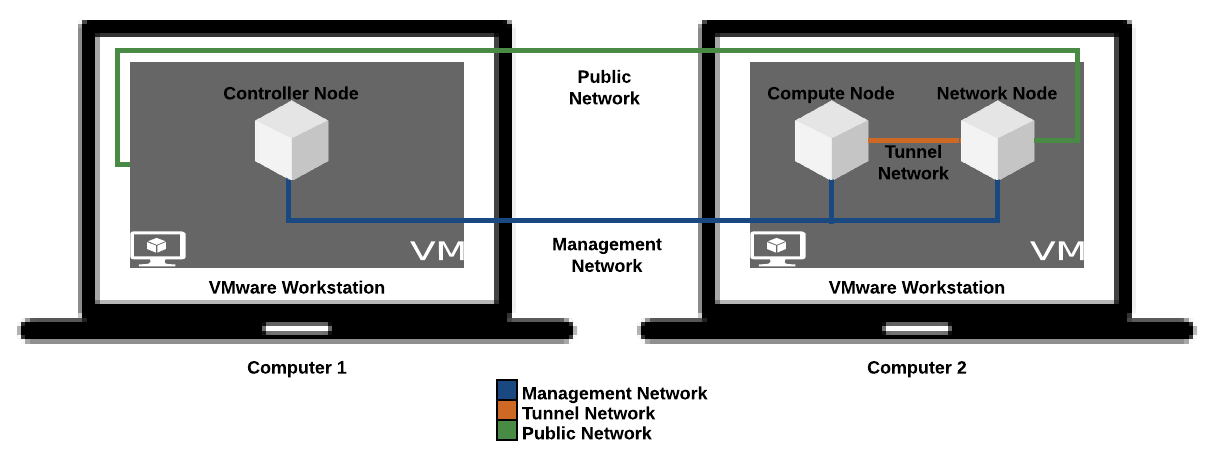
\includegraphics[width=.5\textwidth]{figuras/topologia.png}
	\caption{Topology used in OpenStack installation.}
	\label{fig:topologia}
	\end{figure}
	
% 	Foram criadas duas instâncias (com 512 MB de RAM e sistema operacional CirrOS) na ferramenta como cenário de teste
% 	para os dados serem coletados. 
% 	A topologia utilizada como cenário de teste pode ser vista na Figura \ref{fig:instancias}.
	
	Two instances (using 512MB of RAM and operational system CirrOS) were created in OpenStack as a test scenario to collect data.
	The topology used as test scenario can be seen in Figure \ref{fig:instancias}.
	 
	\begin{figure}[ht]
	\centering
	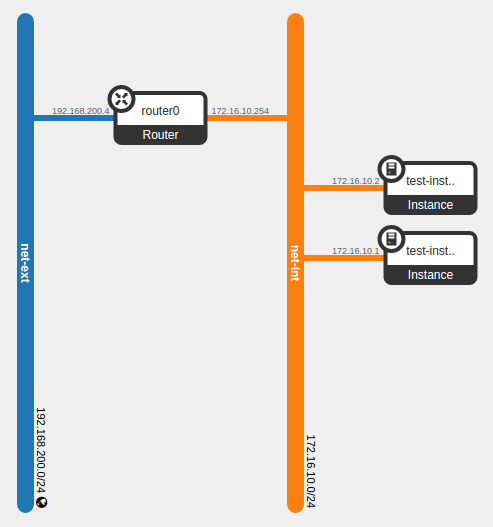
\includegraphics[width=.4\textwidth]{figuras/topologia_teste.png}
	\caption{Topology used as test scenario. {\tiny \textit{Image taken from OpenStack.}}}
	\label{fig:instancias}
	\end{figure}
	
% 	Foi utilizada a versão \textit{Kilo} \cite{openstack_kilo} do OpenStack por ser uma versão estável e mais leve, devido a
% 	limitação dos recursos disponíveis.
% 	Vale ressaltar que apesar do suporte para versão \textit{Kilo} ter sido encerrado pelos mantenedores do OpenStack,
% 	sua arquitetura não distoa muito do seu sucessor subsequente ainda suportado, o OpenStack \textit{Liberty}, o que
% 	não impacta significativamente nem invalida o presente trabalho \cite{openstack_liberty}.
	
	The Kilo \cite{openstack_kilo} version of OpenStack was used because it is a stable and lighter version,
	due to the limited resources available.
	It is worth mentioning that although the support for the Kilo version has been terminated by the OpenStack maintainers,
	its architecture is not far from its subsequent successor, OpenStack Liberty, which does not significantly impact
	or invalidate this work \cite{openstack_liberty}.
		    
    \subsubsection{Obtained results} \label{resultados_levantamento}
  
% 	As métricas foram coletadas por meio do serviço de coleta de dados do OpenStack (módulo - \textit{Ceilometer}) e 
% 	da aplicação \textit{Web} (módulo \textit{Horizon}).
	
	The metrics were collected through the OpenStack data collection service (Ceilometer module) and web application (Horizon module).,
	
% 	Com o cenário de teste realizado as métricas coletadas podem ser vistas na Tabela \ref{tab:metricas_coletadas}.
	
	With the test scenario fulfilled, the collected metrics can be seen in Table \ref{tab:metricas_coletadas}.
	
\begin{table}[h!]
\centering
\caption{Collected metrics in test scenario}
\label{tab:metricas_coletadas}
\begin{tabular}{@{}lcccc@{}}
\toprule
\multicolumn{1}{c}{\textbf{OpenStack metric}}                                     & \textbf{Max} & \textbf{Min} & \textbf{Average} & \textbf{Unit} \\ \midrule
cpu\_util                                                                & 16.11        & 0            & 7.9            & \%               \\
memory                                                                   & 512          & 512          & 512            & MB               \\
memory.usage                                                             & -            & -            & -              & MB               \\
disk.root.size                                                           & 1            & 1            & 1              & GB               \\
vcpus                                                                    & 1            & 1            & 1              & nº vCPUs         \\
\begin{tabular}[c]{@{}l@{}}network.incoming\\ .packets\end{tabular}      & 19           & 8            & 11.75          & packets          \\
\begin{tabular}[c]{@{}l@{}}network.incoming\\ .packets.rate\end{tabular} & 0.0016       & 0.00011      & 0.00011        & packets/s        \\
\begin{tabular}[c]{@{}l@{}}network.outgoing\\ .packets\end{tabular}      & 9            & 9            & 9              & packets          \\
\begin{tabular}[c]{@{}l@{}}network.outgoing\\ .packets.rate\end{tabular} & 0            & 0            & 0              & packets/s        \\
disk.read.requests                                                       & 1122         & 877          & 1032.77        & requests      \\
\begin{tabular}[c]{@{}l@{}}disk.read\\ .requests.rate\end{tabular}       & 0.23         & 0            & 0.015          & requests/s    \\
disk.write.requests                                                      & 134          & 55           & 111.9          & requests      \\
\begin{tabular}[c]{@{}l@{}}disk.write\\ .requests.rate\end{tabular}      & 0.091        & 0            & 0.001          & requests/s    \\
disk.read.bytes                                                          & 20436992     & 18510848     & 20245043.2     & bytes            \\
disk.read.bytes.rate                                                     & 3700.63      & 0            & 206.49         & bytes/s          \\
disk.write.bytes                                                         & 397312       & 206848       & 348262.4       & bytes            \\
disk.write.bytes.rate                                                    & 268.85       & 0            & 22.14          & bytes/s          \\ \bottomrule
\end{tabular}
\end{table}

It is possible to see that OpenStack is a very powerful tool that provides a good service of measurement (Ceilometer module),
being that in a simple scenario (creation of two instances on the tool) several metrics are generated and can be monitored to 
guarantee QoS.


\section{Conclusão}
Com a revisão de literatura realizada foi possível coletar 68 métricas relacionadas a QoS para serviços de nuvem, das quais
35 foram avaliadas no Openstack. Na avaliação foi possível perceber que o Openstack provia aproximadamente 24,25\% das métricas
exatas e, além disso, possuia algumas outras métricas relacionadas com as métricas identificadas.

O número de métricas encontradas deve-se ao fato de que o Openstack possui um módulo apenas para coleta de métricas. 
Os resultados obtidos neste trabalham servem de insumo para outros estudos relacionados e para construção de ferramentas de seleção de 
serviços de nuvem, auxiliando no levantamento das métricas possíveis de serem extraídas do Openstack.

Além do módulo de coleta de dados, o OpenStack oferece alguns mecanismos de garantia de qualidade de serviço. São eles:

\begin{itemize}
 \item Funcionalidade que permite estabelecer limites para tamanhos de arquivos, memória RAM, instâncias, vCPUs;
 \item Funcionalidade que permite criar regras de segurança para limitar tráfegos específicos nas instâncias;
 \item Plugin do Neutron para criar regras de QoS para limitar largura de banda nas instâncias, de modo 
 a garantir uma largura de banda mínima \cite{openstack_neutron} \cite{openstack_neutron_qos};
 \item Projeto Aodh \cite{openstack_telemetry} que provê um serviço de alarme, onde é possível criar regras de monitoramento de métricas para que 
quando um certo limite seja alcançado o usuário seja notificado.
\end{itemize}


Uma limitação identificada do trabalho é que foi considerada uma versão antiga da ferramenta. Outra limitação é que as métricas
foram identificadas por uma revisão simples de literatura, o que não possibilitou uma visibilidade do máximo de trabalhos possíveis,
ou seja, foram considerados poucos estudos relacionados. A análise de apenas métricas nativas sem a consideração de \textit{plugins} e/ou
outras ferramentas também é considerada uma limitação.

Como trabalho futuro é visto a aplicação de uma revisão sistemática com o intuito de encontrar mais métricas e aplicá-las para
uma versão mais atual do Openstack e considerar outras ferramentas.


%%%%%%%%%%%%%%%%%%%%%%%%%%%%%%%%%

% % Propor os requisitos de hardware (RAM, HD) como métrica de QoS

%%%%%%%%%%%%%%%%%%%%%%%%%%%%%%%%%


% \subsection{Subsection Heading Here}
% Subsection text here.
% 
% 
% \subsubsection{Subsubsection Heading Here}
% Subsubsection text here.


% An example of a floating figure using the graphicx package.
% Note that \label must occur AFTER (or within) \caption.
% For figures, \caption should occur after the \includegraphics.
% Note that IEEEtran v1.7 and later has special internal code that
% is designed to preserve the operation of \label within \caption
% even when the captionsoff option is in effect. However, because
% of issues like this, it may be the safest practice to put all your
% \label just after \caption rather than within \caption{}.
%
% Reminder: the "draftcls" or "draftclsnofoot", not "draft", class
% option should be used if it is desired that the figures are to be
% displayed while in draft mode.
%
%\begin{figure}[!t]
%\centering
%\includegraphics[width=2.5in]{myfigure}
% where an .eps filename suffix will be assumed under latex, 
% and a .pdf suffix will be assumed for pdflatex; or what has been declared
% via \DeclareGraphicsExtensions.
%\caption{Simulation results for the network.}
%\label{fig_sim}
%\end{figure}

% Note that the IEEE typically puts floats only at the top, even when this
% results in a large percentage of a column being occupied by floats.


% An example of a double column floating figure using two subfigures.
% (The subfig.sty package must be loaded for this to work.)
% The subfigure \label commands are set within each subfloat command,
% and the \label for the overall figure must come after \caption.
% \hfil is used as a separator to get equal spacing.
% Watch out that the combined width of all the subfigures on a 
% line do not exceed the text width or a line break will occur.
%
% \begin{figure*}[!t]
% \centering
% \subfloat[Case I]{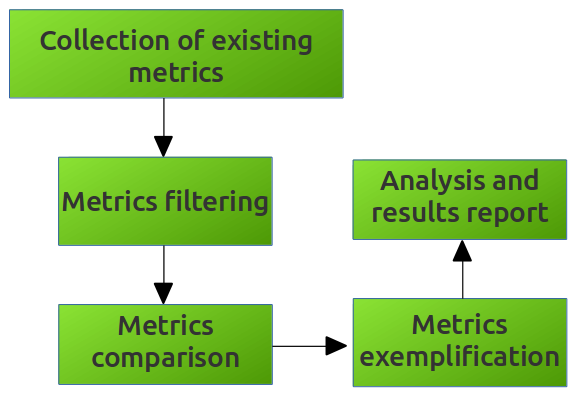
\includegraphics[width=2.5in]{figuras/metodologia}%
% \label{fig_first_case}}
% \hfil
% \subfloat[Case II]{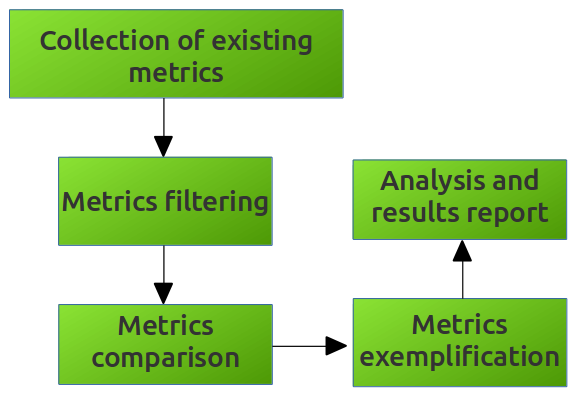
\includegraphics[width=2.5in]{figuras/metodologia}%
% \label{fig_second_case}}
% \caption{Simulation results for the network.}
% \label{fig_sim}
% \end{figure*}
%
% Note that often IEEE papers with subfigures do not employ subfigure
% captions (using the optional argument to \subfloat[]), but instead will
% reference/describe all of them (a), (b), etc., within the main caption.
% Be aware that for subfig.sty to generate the (a), (b), etc., subfigure
% labels, the optional argument to \subfloat must be present. If a
% subcaption is not desired, just leave its contents blank,
% e.g., \subfloat[].


% An example of a floating table. Note that, for IEEE style tables, the
% \caption command should come BEFORE the table and, given that table
% captions serve much like titles, are usually capitalized except for words
% such as a, an, and, as, at, but, by, for, in, nor, of, on, or, the, to
% and up, which are usually not capitalized unless they are the first or
% last word of the caption. Table text will default to \footnotesize as
% the IEEE normally uses this smaller font for tables.
% The \label must come after \caption as always.
%
%\begin{table}[!t]
%% increase table row spacing, adjust to taste
%\renewcommand{\arraystretch}{1.3}
% if using array.sty, it might be a good idea to tweak the value of
% \extrarowheight as needed to properly center the text within the cells
%\caption{An Example of a Table}
%\label{table_example}
%\centering
%% Some packages, such as MDW tools, offer better commands for making tables
%% than the plain LaTeX2e tabular which is used here.
%\begin{tabular}{|c||c|}
%\hline
%One & Two\\
%\hline
%Three & Four\\
%\hline
%\end{tabular}
%\end{table}


% Note that the IEEE does not put floats in the very first column
% - or typically anywhere on the first page for that matter. Also,
% in-text middle ("here") positioning is typically not used, but it
% is allowed and encouraged for Computer Society conferences (but
% not Computer Society journals). Most IEEE journals/conferences use
% top floats exclusively. 
% Note that, LaTeX2e, unlike IEEE journals/conferences, places
% footnotes above bottom floats. This can be corrected via the
% \fnbelowfloat command of the stfloats package.

% conference papers do not normally have an appendix


% use section* for acknowledgment
% \section*{Acknowledgment}


% The authors would like to thank...





% trigger a \newpage just before the given reference
% number - used to balance the columns on the last page
% adjust value as needed - may need to be readjusted if
% the document is modified later
%\IEEEtriggeratref{8}
% The "triggered" command can be changed if desired:
%\IEEEtriggercmd{\enlargethispage{-5in}}

% references section

% can use a bibliography generated by BibTeX as a .bbl file
% BibTeX documentation can be easily obtained at:
% http://mirror.ctan.org/biblio/bibtex/contrib/doc/
% The IEEEtran BibTeX style support page is at:
% http://www.michaelshell.org/tex/ieeetran/bibtex/
%\bibliographystyle{IEEEtran}
% argument is your BibTeX string definitions and bibliography database(s)
%\bibliography{IEEEabrv,../bib/paper}
%
% <OR> manually copy in the resultant .bbl file
% set second argument of \begin to the number of references
% (used to reserve space for the reference number labels box)

% Please add the following required packages to your document preamble:
% \usepackage{multirow}

\bibliographystyle{IEEEtran}
\bibliography{references}
% \begin{thebibliography}{1}
% 
% \bibitem{IEEEhowto:kopka}
% H.~Kopka and P.~W. Daly, \emph{A Guide to \LaTeX}, 3rd~ed.\hskip 1em plus
%   0.5em minus 0.4em\relax Harlow, England: Addison-Wesley, 1999.
% 
% \end{thebibliography}




% that's all folks
\end{document}


